\documentclass[12pt]{article}
\usepackage[utf8]{inputenc}
\usepackage[spanish]{babel}
\usepackage{float}
\usepackage{graphicx}
\usepackage{fancyhdr}
\usepackage{graphics}
\usepackage[
    type={CC},
    modifier={by-nc-sa},
    version={4.0},
]{doclicense}
\usepackage{mdframed}
\usepackage[margin = 1.2in]{geometry}
\usepackage{listings} 
\usepackage{color}
\usepackage[listings]{tcolorbox}

\definecolor{codegreen}{rgb}{0,0.6,0} \definecolor{codegray}{rgb}{0.5,0.5,0.5} \definecolor{codepurple}{rgb}{0.58,0,0.82} \definecolor{backcolour}{rgb}{0.95,0.95,0.92}

\lstdefinestyle{mystyle}{ backgroundcolor=\color{backcolour}, commentstyle=\color{ codegreen}, 
keywordstyle=\color{magenta}, numberstyle=\tiny\color{codegray}, stringstyle=\color{codepurple}, 
basicstyle=\footnotesize,
breakatwhitespace=false,
breaklines=true,
captionpos=b,
keepspaces=true,
numbers=left,
numbersep=5pt,
showspaces=false,
showstringspaces=false,
showtabs=false,
tabsize=2
}

\lstset{style=mystyle}


\title{Guía del auto-Hacker Galáctico}
\author{Fernando Méndez Torrubiano}
\date{\today}

\begin{document}
\pagestyle{fancy} %Estilo de página a partir de aquí
\rhead{Guía del auto-Hacker Galáctico} %Encabezado a la derecha.
\lhead{Fernando Méndez}

\maketitle

\begin{figure}[H]
    \centering
    
\includegraphics[width= 0.75\textwidth]{Media/portada.png}
\end{figure}

%\begin{figure}[H]
%    \centering
%    
\includegraphics[width= 0.8\textwidth]{Media/logo.jpg}
%\end{figure}

%\begin{figure}[H]
%    \centering
%    
\includegraphics[width= 0.8\textwidth]{Media/bandera.jpg}
%\end{figure}

\newpage
\tableofcontents

\newpage
\section{Introducción}
Bienvenidos a la \testxtbf{Guía del auto-Hacker Galáctico}, un breve documento en el que se explicarán las nociones básicas para comenzar tu camino como \textit{hacker} en \textbf{FDIst}.
\newline
\noindent
\subsection{Sistemas Operativos}
\noindent
He de comenzar diciendo que todo lo que se explique aquí, irá enfocado a la plataforma \testxtbf{Linux}, sin embargo, si usas \textbf{Windows}, no te preocupes, pues te enseñaremos a crear y usar una máquina virtual para que puedas trabajar sin necesidad de tener ninguna distribución de \textbf{GNU/Linux}.
\newline\\
Además, recalcar que cada uno es libre de usar la plataforma en la que más cómodo se sienta, no por usar \textbf{Windows o MacOS}, serás un informático de segunda, las herramientas están ahí y gracias a internet, toda la documentación está a vuestro alcance. Por tanto, si preferís usar otro Sistema Operativo (SO), que no esté basado en GNU/Linux, sabed que tenéis herramientas equivalentes a las que se van a detallar en esta guía. Eso sí, \textbf{tened cuidado con qué instaláis}, pues existen programas de dudosa seguridad y que incluyen spyware.
\subsection{Advertencia y VPN}
\noindent
Por último advertíos de que \textbf{FDIst} tiene un acuerdo con el \textbf{CERN}, el \textbf{CSN} y el \textbf{Centro de Procesamiento de Datos (CPD)} de la Universidad Complutense de Madrid (UCM). Cualquier ataque a otra entidad o empresa, no estará respaldado por FDIst y \textbf{todo ataque que se realice a los centros anteriormente mencionados, deberá ser a través de la VPN} que se os proporcionará en este mismo manual y a la que previamente se os habrá dado acceso a través de vuestro correo UCM.
\newpage
\section{Instalación de Linux}
En primer lugar, \textbf{si NO queréis instalar Linux}, porque no lo vais a usar para nada más, a parte de las actividades de FDIst, os recomiendo \textbf{leer el apartado \textit{2.1}}, saltaros el resto e ir al punto \textbf{\textit{3.Instalación de una Máquina Virtual en Windows}}.

\subsection{Elección de la distribución}
Existen múltiples distribuciones de Linux, nosotros os haremos una \textbf{lista de recomendaciones basadas en Debian y Arch}, pero podéis descargar la que más os guste:
\begin{itemize}
    \item \textbf{Ubuntu}: Es la más popular y no es casualidad, pues esta distribución se creó para llevar Linux al público en general. Es la más sencilla de usar y la que dispone de un entorno más familiar, por contra, es de las que peor rendimiento tiene.
    \newline Podéis descargar la última versión desde su página oficial: \newline \url{https://ubuntu.com/download/desktop}. 
    
    \item \textbf{Ubuntu Mate}: Una de mis favoritas, pues está pensada para equipos con peores prestaciones que Ubuntu, sin embargo, mantiene ese entorno familiar para los usuarios poco experimentados.
    \newline Podéis descargar la última versión desde su página oficial: \newline \url{https://ubuntu-mate.org/download/}.
    
    \item \textbf{Linux Mint}: Ligero y fácil de usar. Esa es la filosofía que marca a esta distribución, muy recomendada para equipos modestos y para amantes de Windows.
    \newline Podéis descargar la última versión desde su página oficial: \newline \url{https://linuxmint.com/download.php}.
     
    \item \textbf{Manjaro}: Bueno, bonito y gratis, pero no es tan sencillo de instalar como el resto de distribuciones. Si es la primera vez que instaláis Linux os costará, si no, esta distribución os encantará.
    \newline Podéis descargar la última versión desde su página oficial: \newline \url{https://manjaro.org/download/}.
     
    \item \textbf{Raspbian}: No es mala idea tener una Raspberry Pi conectada en casa y hacer ataques desde la FDI, conectado a ella mediante SSH (es lo que hago yo), para ello, os recomendamos el SO, creado exclusivamente para esta plataforma.
    \newline Podéis descargar la última versión desde su página oficial: \newline \url{https://www.raspberrypi.org/downloads/}.
     
    \item \textbf{Debian}: Por qué hablar de distribuciones para Debian, si tenemos el propio Debian. El \textit{sistema operativo universal}, no apto para \textit{noobs}. Realmente, sólo te recomendamos instalar este SO, si tienes experiencia en la plataforma Linux.
    \newline Podéis descargar la última versión desde su página oficial: \newline \url{https://www.debian.org/distrib/netinst}.
   
\end{itemize}

\subsection{Preparación de la unidad de instalación}
Una vez elegida nuestra distribución favorita y descargada la imagen de la misma (.ISO), podremos pasar a instalarla.
\newline\\ Para ello necesitaremos lo siguiente:
\begin{itemize}
    \item Un \textbf{PenDrive} de al menos 8Gb (en algunos casos valdrá con menos capacidad).
    \item La \textbf{ISO} descargada de la distribución que queramos instalar.
    \item El programa \textbf{RUFUS}, para la preparación del PenDrive. 
    \newline Lo podéis descargar desde esta página: \url{https://rufus.ie/}
\end{itemize}

\noindent Preparación de la unidad USB (Advertencia, la unidad se formateará y se perderá toda la información contenida en su interior, por favor, realiza una copia de seguridad de tus archivos):
\begin{enumerate}
    \item Introducimos la unidad USB en el PC donde hayamos descargado la ISO e iniciamos RUFUS.
    \item Pulsamos \textit{SELECCIONAR} y buscamos la el archivo ISO en la página donde lo hayamos guardado.
    \begin{figure}[H]
        \centering
        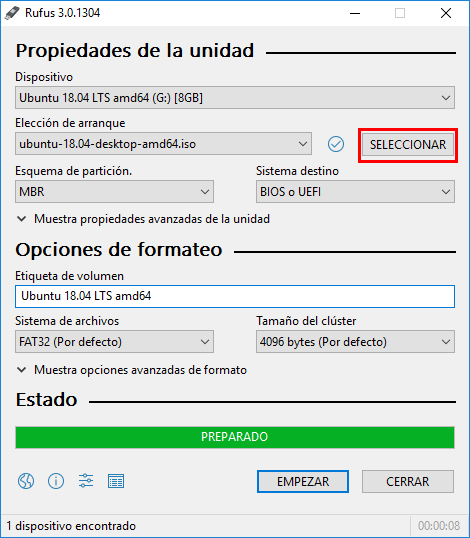
\includegraphics[width= 0.4 \textwidth]{Media/rufus_es_ISO.png}
    \end{figure}
    \newpage
    \item Pulsamos \textit{EMPEZAR} y esperamos al que el programa prepare la unidad. Una vez finalizado, \textbf{extraemos el pendrive con srguridad} y listo.
    \begin{figure}[H]
        \centering
        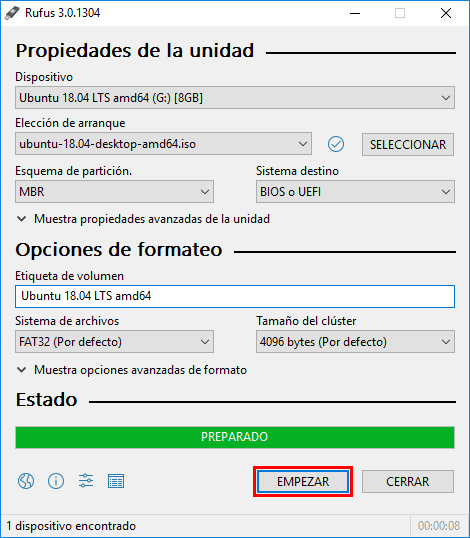
\includegraphics[width= 0.4 \textwidth]{Media/rufus_es_empezar.png}
    \end{figure}
\end{enumerate}

\subsection{Arrancar el instalador del sistema}
\begin{enumerate}
    \item Introducimos la unidad de instalación USB que hemos preparado anteriormente en el ordenador en el que queramos instalar el SO.
    \item Si en la BIOS no tenemos seleccionado que la unidad de arranque primaria sea el USB, pulsaremos rápidamente F12 hasta que nos aparezca el \textit{"Boot Menu"} (en algunas placas base puede variar, consultar en la web oficial del fabricante).
    \item Seleccionamos el USB como unidad de arranque y se iniciará el instalador de la distribución de Linux elegida.
    \begin{figure}[H]
        \centering
        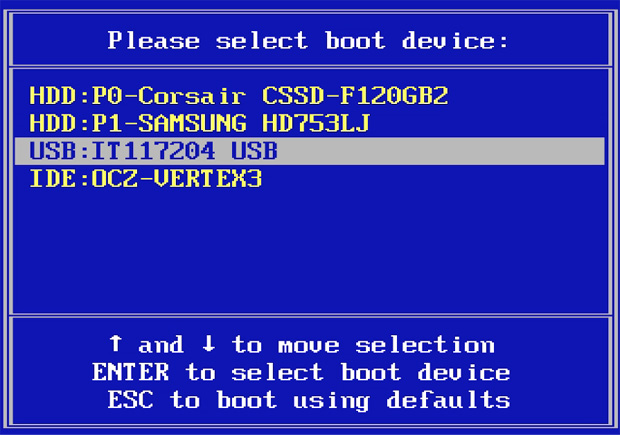
\includegraphics[width= 0.5 \textwidth]{Media/boot-menu-formatear-pc.jpg}
    \end{figure}
\end{enumerate}

\subsection{Opciones de instalación}
    \subsubsection{Idioma} 
    Seleccionamos el idioma que deseemos para el sistema y pulsamos en \textit{'Continuar'}.
     \begin{figure}[H]
        \centering
        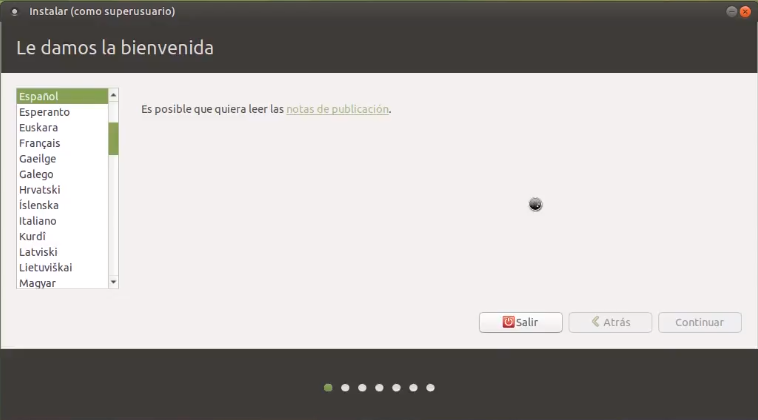
\includegraphics[width= 0.7 \textwidth]{Media/umate1.png}
    \end{figure}
    \subsubsection{Distribución de teclado}
    Seleccionamos la distribución de teclado que queramos (aseguraos de que la distribución seleccionada es la \textbf{ESPAÑOLA}, si no luego tendréis muchos problemas a la hora de escribir) y pulsamos en \textit{'Continuar'}.
     \begin{figure}[H]
        \centering
        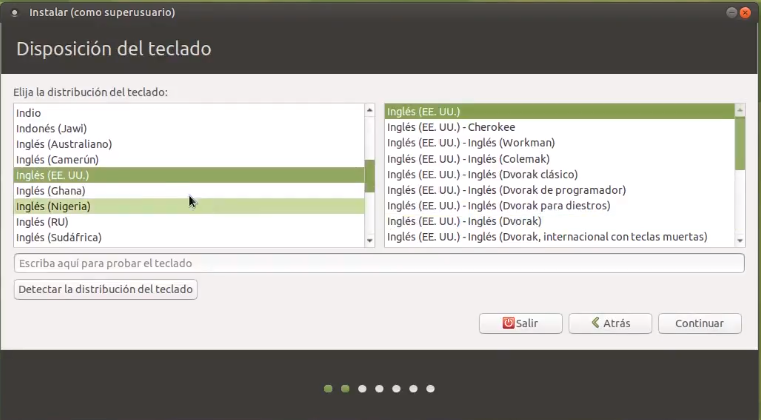
\includegraphics[width= 0.7 \textwidth]{Media/umate2.png}
    \end{figure}

\newpage    
\subsubsection{Programas y drivers} 
    A continuación nos aparecerán una serie de opciones:
     \begin{figure}[H]
        \centering
        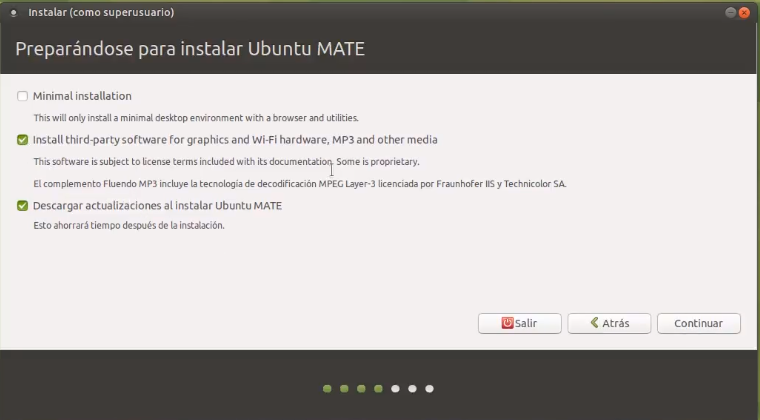
\includegraphics[width= 0.7 \textwidth]{Media/umate3.png}
    \end{figure}
    \begin{itemize}
        \item \textbf{Instalación mínima}: esta opción es recomendable si vamos a instalar Linux junto con Windows y queremos dedicar poco espacio a la partición de Linux. Al seleccionar esta opción, se nos instalarán los programas básicos del sistema y nos ahorraremos espacio, pues no se instalarán herramientas como \textit{LibreOffice} que no utilizaremos.
        \item \textbf{Instalación de software de terceros}: Importante marcar esta opción, pues descargará e instalará drivers que puedan necesitar componentes de nuestro hardware, como los de la tarjeta de red inalámbrica o nuestra tarjeta gráfica.
        \item \textbf{Descargar actualizaciones al instalar}: Opcional, pero recomendado marcarlo, la instalación tardará unos minutos más, pero luego no tendremos que buscar la última actualización manualmente.
    \end{itemize}
   
    Cuando hayamos seleccionado las opciones que deseemos, pulsamos en \textit{'Continuar'}.
    
\subsubsection{Tipo de instalación}
Ahora es el momento de decidir si queremos instalar Linux junto con Windows, o por el contrario, formatear la unidad e instalar únicamente Linux (borrando Windows de forma permanente.
\begin{figure}[H]
        \centering
        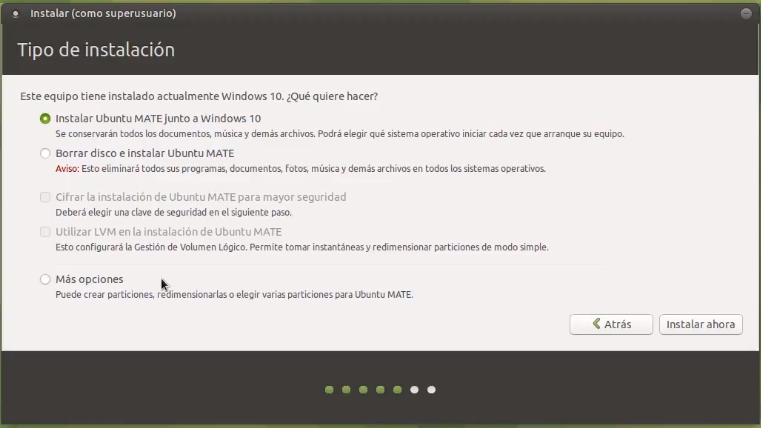
\includegraphics[width= 0.7 \textwidth]{Media/umate4.png}
\end{figure}

\begin{itemize}
    \item \textbf{Instalar Linux junto a Windows}: Esta opción creará automáticamente una partición en nuestro disco duro, donde instalará la distribución de Linux, conservando Windows. Al arrancar el equipo, el GRUB de Linux nos permitirá elegir que sistema arrancar (por defecto pondrá Linux, pero más tarde, podremos modificar el orden de arranque si por defecto queremos poner Windows).
    \item \textbf{Borrar disco e instalar Linux}: Formateará por completo la unidad, eliminará Windows y todos los archivos que contenga, perderemos la licencia del SO.
    \newline \textit{Si seleccionamos esta opción, se nos habilitarán las siguientes opciones}:
    \item \textbf{Cifrar la instalación de Linux para mayor seguridad}: Esto hará que los datos contenidos en el disco sean cifrados, la instalación tardará un poco más y tendrá un impacto en el rendimiento del equipo, por tanto, si tenemos un ordenador con componentes de baja calidad, no es recomendable. Por el contrario, si queremos proteger muy bien nuestros archivos, entonces es recomendable seleccionar esta opción.
    \item \textbf{Utilizar LVM}: Esto no es más que un sistema que administración de discos, es recomendable seleccionar esta opción, pues en un futuro puede que queramos volver a instalar Windows o otra distribución de Linux junto con la actual.
\end{itemize}
Por otra parte, si queremos instalar Linux junto con Windows, pero queremos seleccionar nosotros mismos el espacio que se le dedica a cada Sistema Operativo, seleccionaremos la siguiente opción:
\begin{itemize}
    \item \textbf{Más opciones}: Nos permitirá crear la partición de Linux con el tamaño que queramos, ajustando así, cuánto espacio del disco le dejamos a Windows. Es recomendable usar al menos 30GB para la mayoría de distribuciones de Linux, aunque con menos podrían funcionar.
\end{itemize}
Por último, pulsamos en \textit{'Instalar ahora'}.

\subsubsection{Zona horaria}
Seleccionaremos la región donde nos encontremos, en nuestro caso, Madrid. Y pulsamos en \textit{'Continuar'}.
\begin{figure}[H]
        \centering
        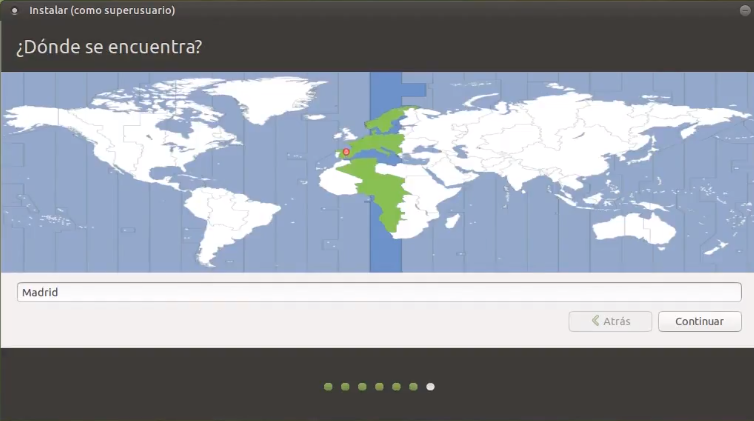
\includegraphics[width= 0.7 \textwidth]{Media/umate5.png}
\end{figure}

\subsection{Usuario y contraseña}
Por último, le asignaremos un nombre al equipo, crearemos el usuario con el nombre que queramos e creamos una nueva contraseña. Si queremos podemos seleccionar la opción de \textit{'Iniciar sesión automáticamente'}, para que no nos pida nuestra contraseña al iniciar nuestro ordenador (más cómodo, pero mucho más inseguro). 
\newline Pulsamos en \textit{'Continuar'} y comenzará la instalación.
\begin{figure}[H]
        \centering
        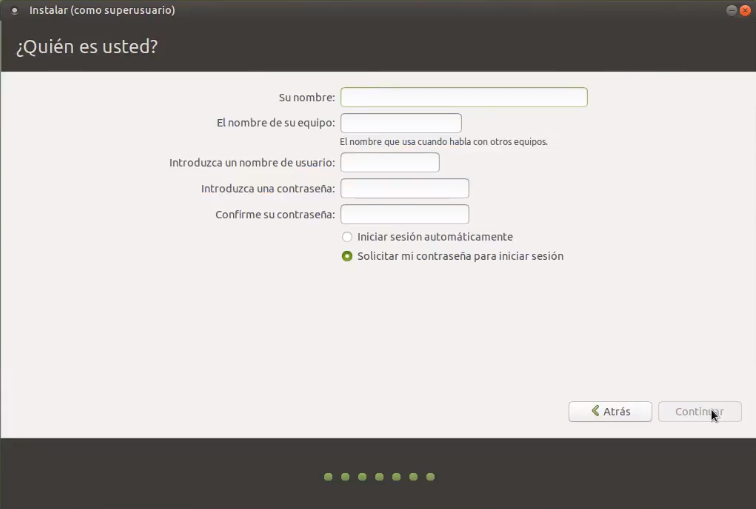
\includegraphics[width= 0.7 \textwidth]{Media/umate6.png}
\end{figure}

\newpage
\subsection{Finalizar la instalación}
Cuando la instalación finalice, nos aparecerá un nuevo cuadro de diálogo, en el que pulsaremos en \textit{'Reiniciar ahora'} y ya podremos comenzar a usar nuestra distribución de Linux.
\begin{figure}[H]
        \centering
        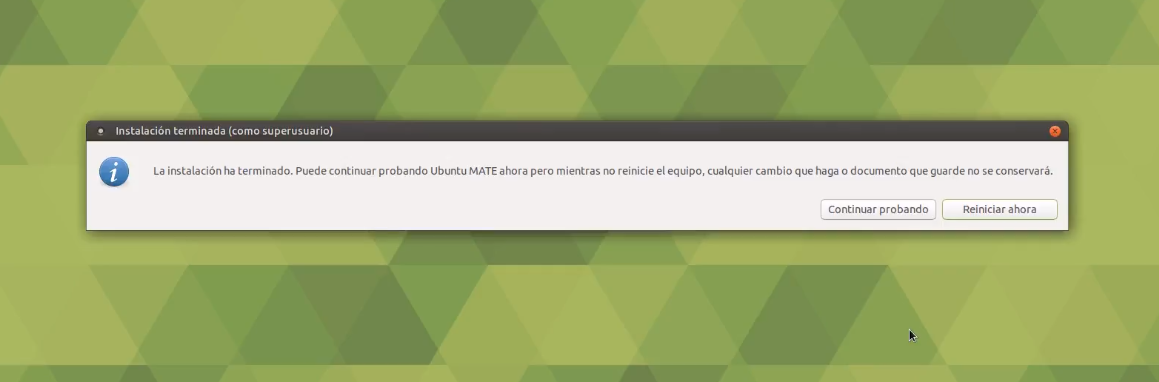
\includegraphics[width= 0.7 \textwidth]{Media/umate7.png}
\end{figure}

\subsubsection{Poner Windows como primera opción del GRUB}
Como habremos observado, al reiniciar el equipo (si hemos instalado Linux junto con Windows, nos aparecerá la ventana en la que nos permite escoger que SO iniciar.
\newline Por defecto viene seleccionada la distrubución de Linux que hayamos instalado y hay una cuenta atrás que iniciará está automáticamente, a no ser que toquemos alguna flecha del teclado para seleccionar otra opción.
\begin{figure}[H]
        \centering
        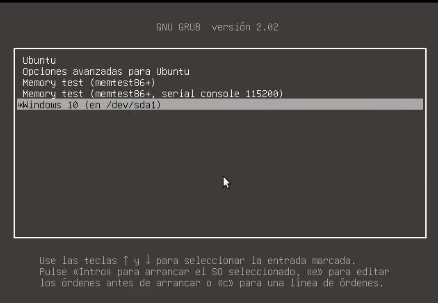
\includegraphics[width= 0.7 \textwidth]{Media/grub.png}
\end{figure}
\newline A continuación os explico cómo poner Windows por defecto:
\begin{enumerate}
    \item Abriremos una terminal desde nuestra distribución de Linux y escribiremos el siguiente comando: \textbf{sudo nano /boot/grub/grub.cfg}
    \item Se nos abrirá un documento editable como este:
    \begin{figure}[H]
        \centering
        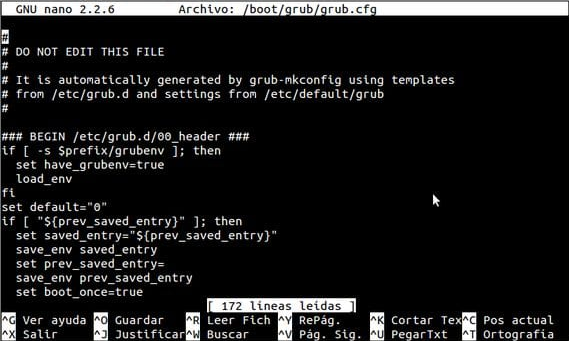
\includegraphics[width= 0.7 \textwidth]{Media/grubload.png}
    \end{figure}
    En donde tendremos que modificar sólo la linea \textbf{\verb=set default='0'}. Cambiando el '0' por el '4', que es el número que, en mi caso, corresponde a la partición de Windows que esta instalada junto a tu sistema Linux.
    \item Hecho esto, pulsamos 'CTRL+X' para salir, pulsamos la tecla 'S' para guardar y a continuación la tecla 'ENTER' para confirmar.
\end{enumerate}
Y listo, la próxima vez que iniciemos el equipo, Windows será la opción por defecto.
\newpage
\section{Máquina Virtual de Linux en Windows}
Aunque vayamos a utilizar una máquina virtual, \textbf{es necesario tener una ISO de la distribución de Linux que queramos usar}.
\newline Para ello, os recomiendo leer el apartado \textbf{\textit{2.1. Elección de la distribución}}.
\newline\\
\noindent
Cuando tengamos la ISO, debemos descargar el programa VirtualBox (de Oracle), aunque existen muchos e incluso Windows dispone de forma nativa de un método de virtualización, creemos que VirtualBox es el que mejor funciona:
\newline \url{https://www.virtualbox.org/}

\subsection{Creación de una Máquina Virtual}
\noindent
Una vez instalado VirtualBox, procedemos a crear una máquina virtual.
\newline Para ello pulsamos sobre el icono \textit{'NUEVA'}.
    \begin{figure}[H]
        \centering
        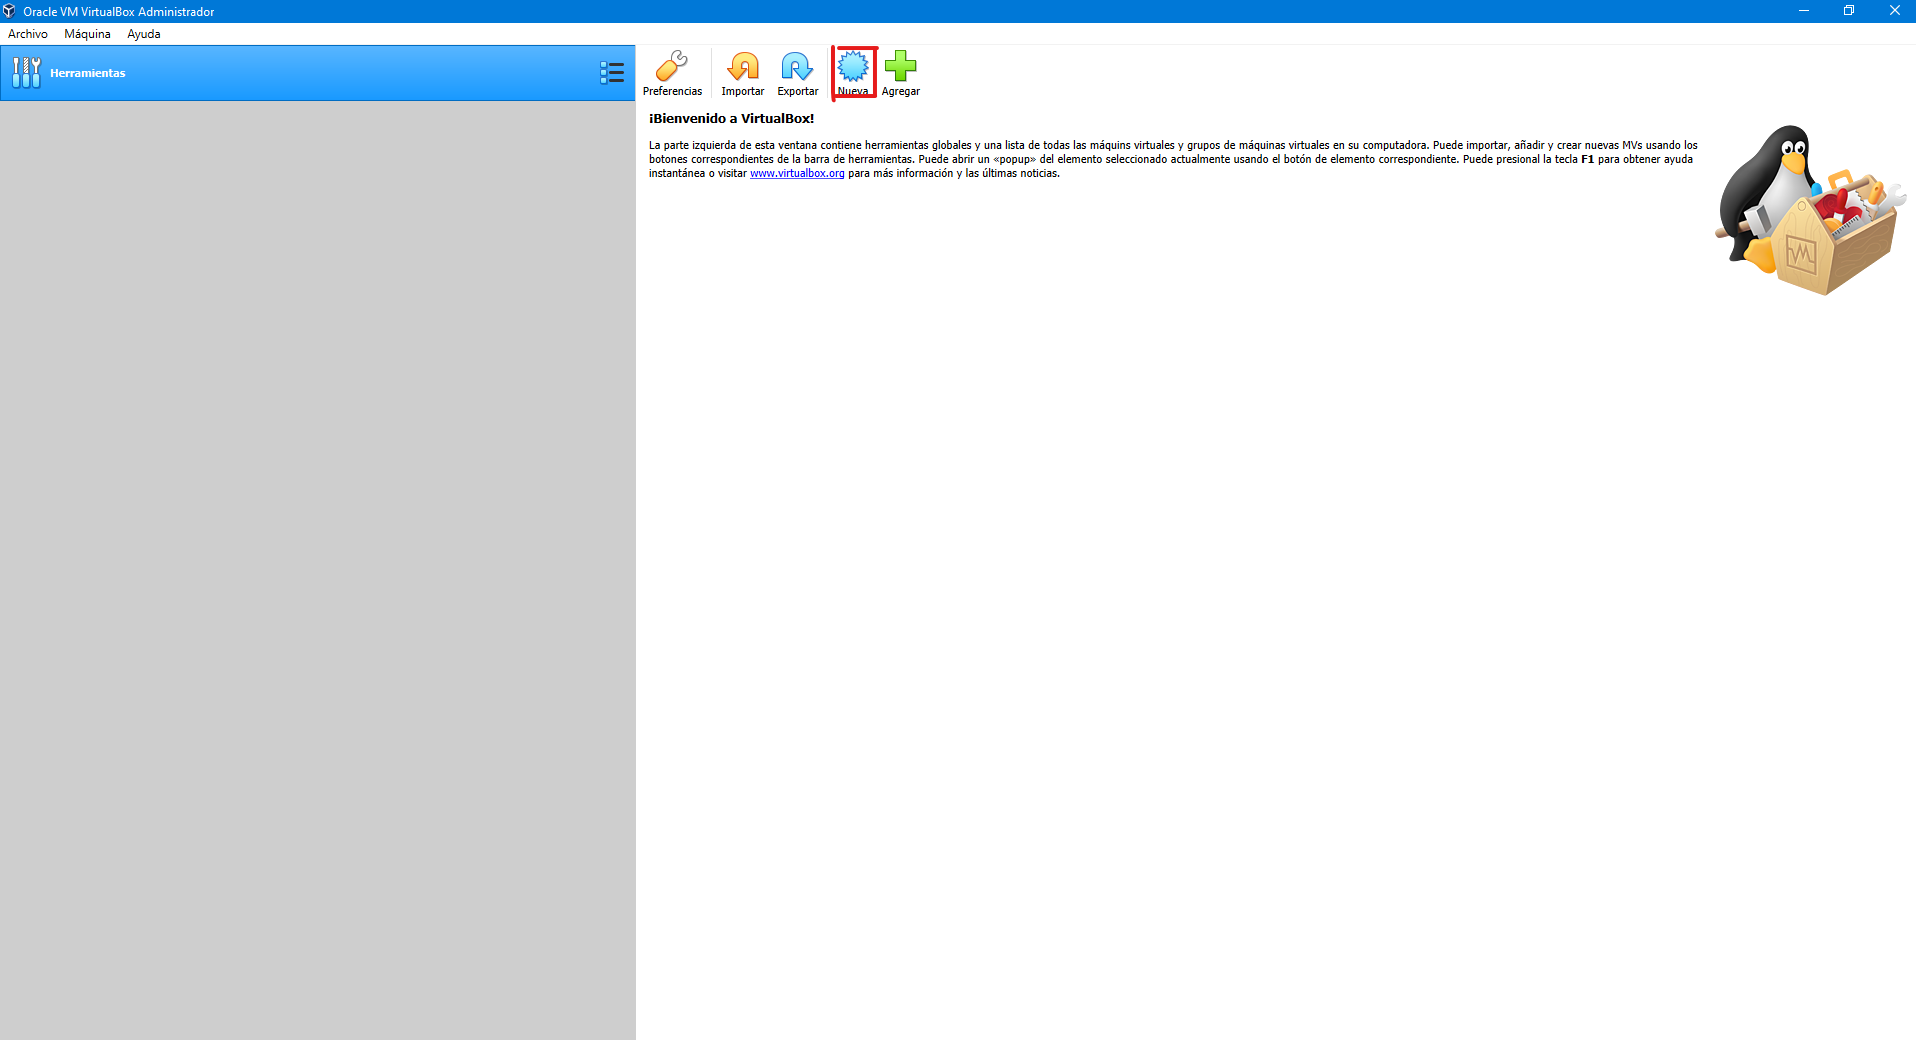
\includegraphics[width= 0.7 \textwidth]{Media/VB1.png}
    \end{figure}
    
\subsection{Configuración Inicial}
\noindent
A continuación daremos un nombre a nuestra Máquina Virtual, seleccionaremos la carpeta donde la vamos a crear y escogeremos el tipo de máquina (en nuestro caso Linux) y su versión (la distribución principal a la que corresponda, en nuestro caso ARCH Linux, pues instalaremos Manjaro).
    \begin{figure}[H]
        \centering
        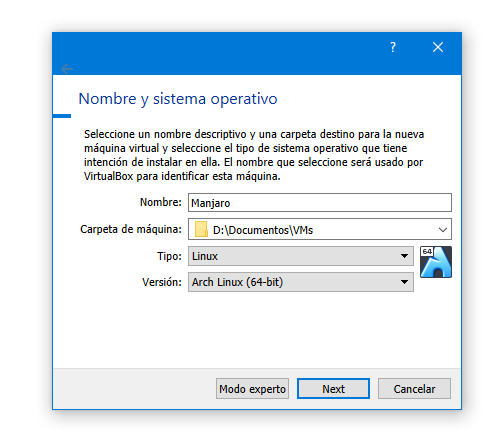
\includegraphics[width= 0.7 \textwidth]{Media/VB2.png}
    \end{figure}
\newline \noindent Pulsamos sobre el botón \textit{'Siguiente'}.

\subsection{Tamaño de la memoria}
\noindent
Ahora seleccionaremos el tamaño de memoria RAM que queremos asignar a nuestra Máquina Virtual. Por defecto nos pone 1024MB, yo os recomiendo subir al menos a 2048MB si vuestro PC tiene 8GB o más de memoria RAM instalada. Tened en cuenta que debéis dejar memoria suficiente para que Windows administre el resto del sistema.
    \begin{figure}[H]
        \centering
        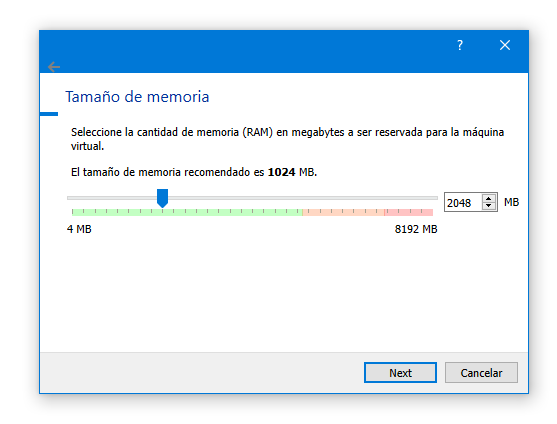
\includegraphics[width= 0.7 \textwidth]{Media/VB3.png}
    \end{figure}
\newline \noindent Pulsamos sobre el botón \textit{'Siguiente'}.

\subsection{Creación de un Disco Duro Virtual}
\noindent
\subsubsection{Creación}
Nuestra máquina necesita estar alojada en algún espacio físico, para ello crearemos una pequeña partición en nuestro disco (un Disco Duro Virtual).
\begin{figure}[H]
        \centering
        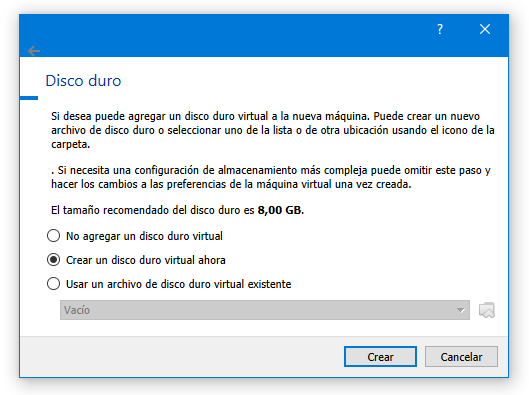
\includegraphics[width= 0.7 \textwidth]{Media/VB4.png}
    \end{figure}
\newline \noindent Pulsamos sobre el botón \textit{'Crear'}.

\subsubsection{Tipo de Disco Duro}
\noindent
VirtualBox nos ofrece 3 opciones, de las cuales, tanto la primera (\textit{VirtualBox Disk Image}, como la segunda (\textit{Virtual Hard Disk}, son recomendables. Lo dejamos a vuestra elección.
\begin{figure}[H]
        \centering
        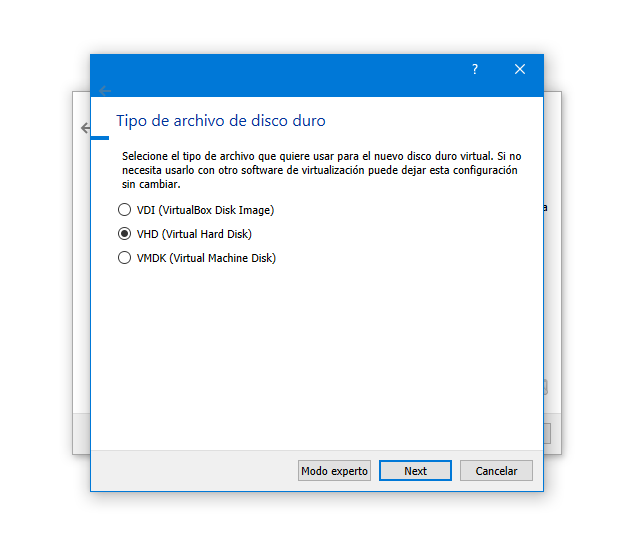
\includegraphics[width= 0.7 \textwidth]{Media/VB5.png}
    \end{figure}
\newline \noindent Pulsamos sobre el botón \textit{'Siguiente'}.

\subsubsection{Tipo de Almacenamiento}
\noindent
En este caso, VirtualBox nos ofrece 2 opciones:
\begin{enumerate}
    \item Reservado dinámicamente: esto irá ocupando espacio en nuestro disco según la Máquina Virtual necesite, hasta el máximo que le asignaremos a continuación.
    \item Tamaño fijo: reservará directamente todo el espacio que le digamos a continuación, tanto si la Máquina Virtual lo está usando, como si no.
\end{enumerate}
\begin{figure}[H]
        \centering
        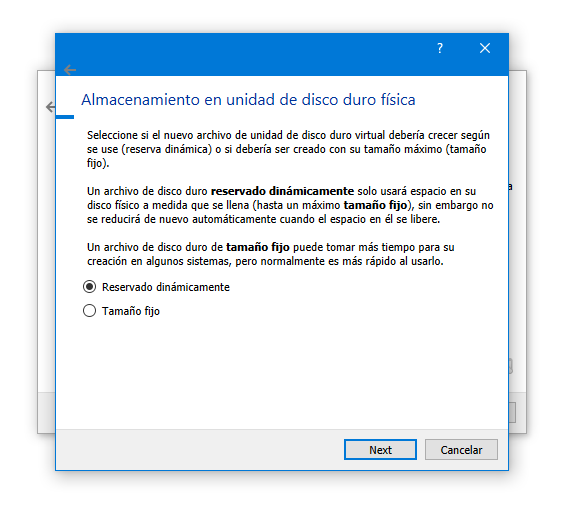
\includegraphics[width= 0.7 \textwidth]{Media/VB6.png}
    \end{figure}
\newline \noindent Pulsamos sobre el botón \textit{'Siguiente'}.

\subsubsection{Ubicación y tamaño}
\noindent
En este apartado podremos seleccionar la ubicación en la que se creará el Disco Duro Virtual. Además, VirtualBox nos recomienda el tamaño mínimo para que la Máquina Virtual funcione, podemos asignar más si así lo queremos.
\begin{figure}[H]
        \centering
        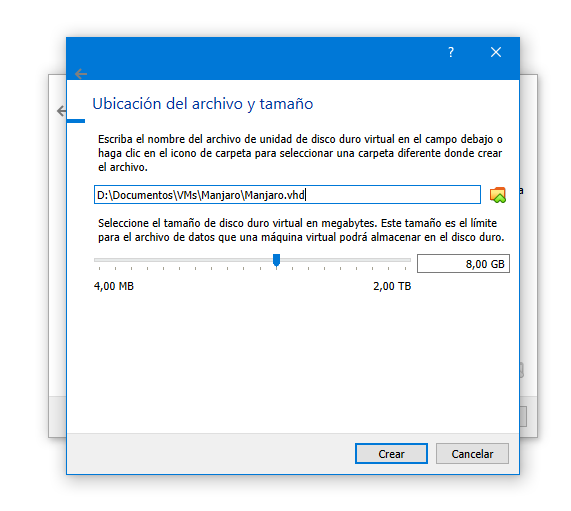
\includegraphics[width= 0.7 \textwidth]{Media/VB7.png}
    \end{figure}
\newline \noindent Pulsamos sobre el botón \textit{'Crear'}.

\subsection{Selección de la ISO}
\noindent
Ahora vamos a decirle a VirtualBox de dónde tiene que leer la ISO para instalar la Máquina Virtual.
\begin{figure}[H]
        \centering
        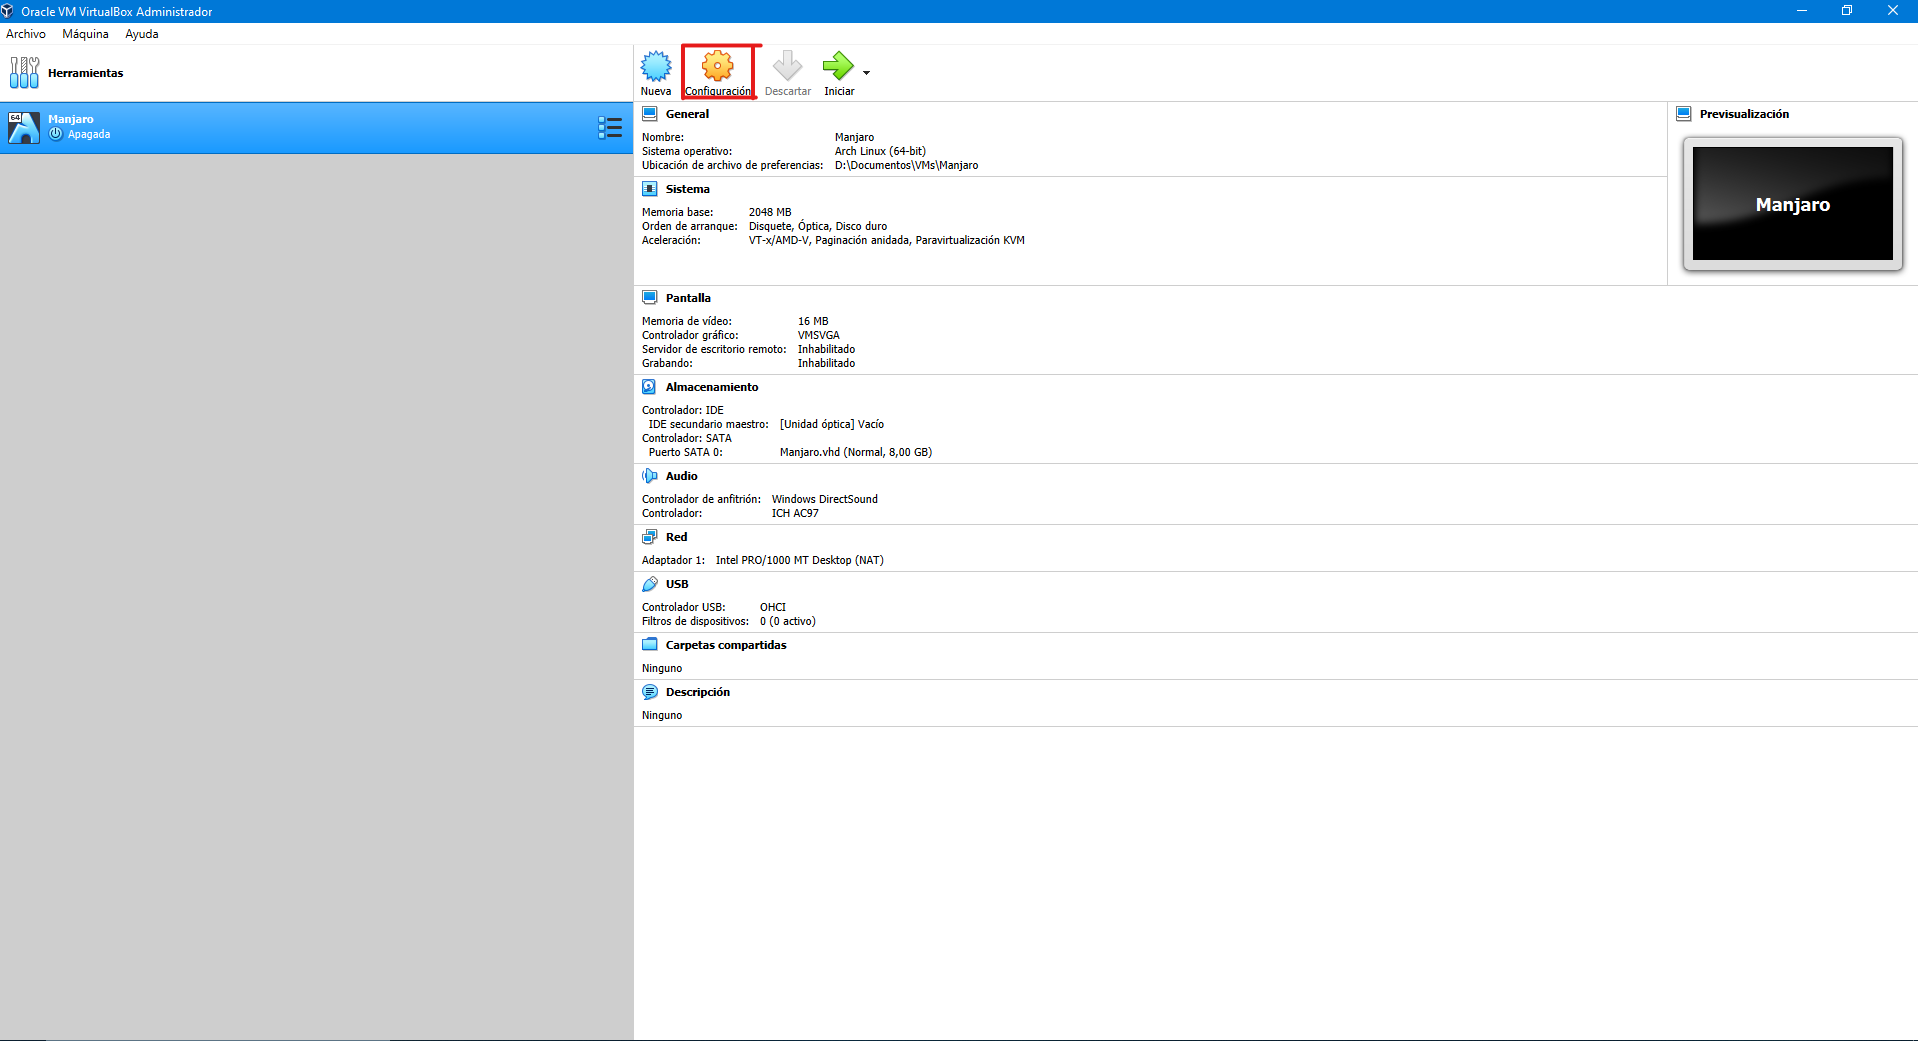
\includegraphics[width= 0.7 \textwidth]{Media/VB8.png}
    \end{figure}
\newline \noindent Pulsamos sobre el botón \textit{'Configuración'}.
\begin{figure}[H]
        \centering
        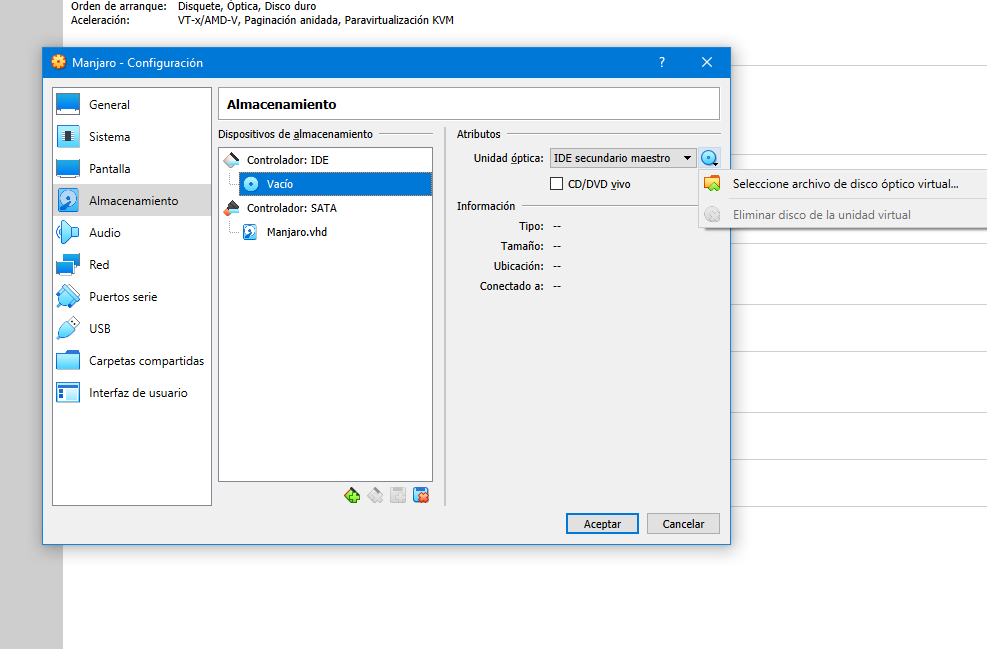
\includegraphics[width= 0.7 \textwidth]{Media/VB9.png}
    \end{figure}
\newline \noindent Vamos a la sección de \textit{'Almacenamiento'} y en el \textit{'Controlador'}, seleccionamos el archivo de disco óptico virtual (lo que sería el medio de instalación).
\begin{figure}[H]
        \centering
        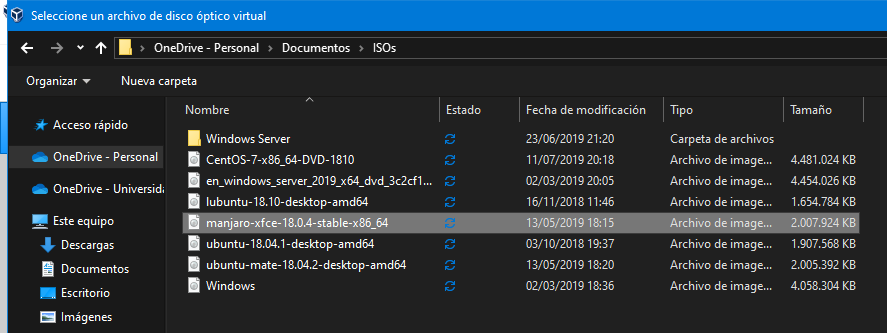
\includegraphics[width= 0.7 \textwidth]{Media/VB10.png}
    \end{figure}
\newline \noindent Buscamos la carpeta donde habíamos guardado la ISO y la seleccionamos.
\begin{figure}[H]
        \centering
        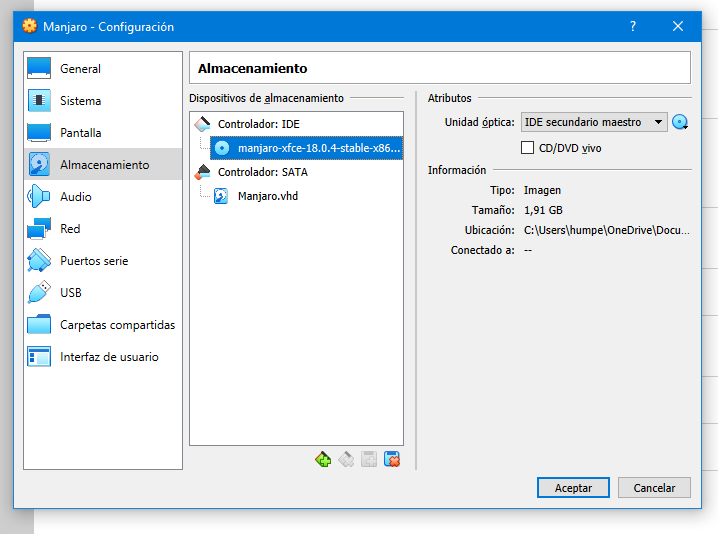
\includegraphics[width= 0.7 \textwidth]{Media/VB11.png}
    \end{figure}
\newline \noindent Pulsamos sobre el botón \textit{'Aceptar'} y listo.
\begin{figure}[H]
        \centering
        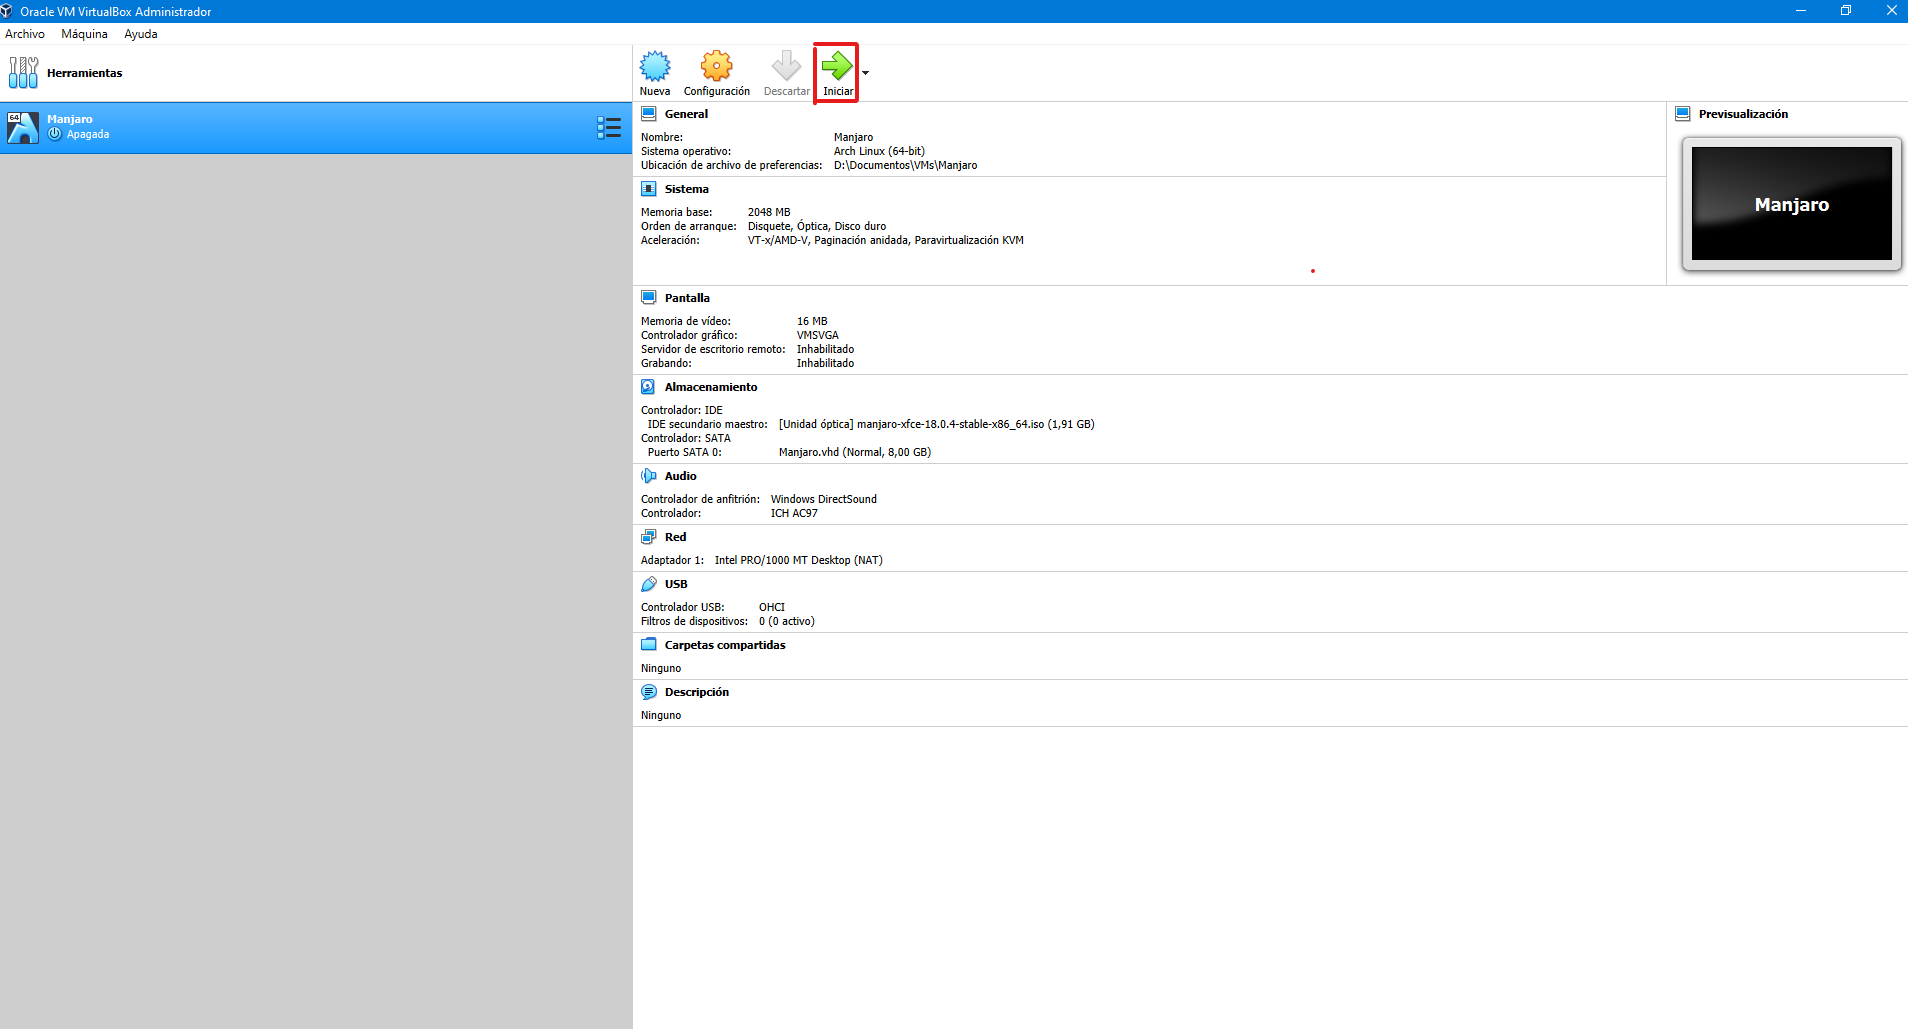
\includegraphics[width= 0.7 \textwidth]{Media/VB12.png}
    \end{figure}
\newline \noindent Ahora ya sólo tenemos que pulsar sobre el botón \textit{'Iniciar'} de la Máquina Virtual y comenzará la instalación. Para guiaros, podéis seguir la guía de instalación del apartado \textbf{\textit{2.Instalación de Linux}}, a partir del punto \textbf{\textit{2.4.Opciones de Instalación}}.

\newpage
\section{Conexión a la VPN, \textsc{HackTheCERN / HackTheCSN / HackTheUCM}}
\subsection{Código ético}
Antes de comenzar, os adjuntamos el \textit{Manual de Código Ético} proporcionado por el \textbf{CERN} y por el \textbf{CSN}. Es muy recomendable que les echéis un vistazo, pues explica las direcciones IPs a las que debéis enfocar vuestros ataques y cómo debéis realizar estos mismos:
\begin{tcolorbox}
    \url{https://cv4.ucm.es/moodle/pluginfile.php/4672494/mod_resource/content/1/CERNCodeOfEthics.pdf}
\end{tcolorbox} 

\begin{tcolorbox}
    \url{https://cv4.ucm.es/moodle/pluginfile.php/7094461/mod_resource/content/1/CodigoEtico.pdf}
\end{tcolorbox} 

\subsection{Registro}
Para poder tener acceso a la VPN, \textbf{es necesario que rellenéis este formulario} con vuestra cuenta UCM y esperéis una confirmación mediante correo electrónico de que se os ha concedido acceso, \textbf{hasta entonces, no podréis realizar ningún ataque}.
\begin{tcolorbox}
    \url{https://fdist.ucm.es/registro/}
\end{tcolorbox}

\subsection{Configuración de la VPN}
\subsubsection{En distribuciones Linux} 
\begin{tcolorbox}[colframe=black!75!blue]
\begin{center}
    (Basadas en Debian: Ubuntu, Linux Mint, Raspbian...)
\end{center}
\end{tcolorbox}
\begin{enumerate}
    \item Abrimos un terminal y escribimos el siguiente comando: 
        \begin{center}
         \textbf{sudo apt-get install vpnc network-manager-vpnc} 
        \end{center}
        \item Si tenemos un escritorio basado en GNOME, escribiremos: 
        \begin{center}
         \textbf{sudo apt-get install network-manager-vpnc-gnome}
        \end{center}
\end{enumerate}

\begin{tcolorbox}[colframe=black!75!red]
\begin{center}
    (En otras versiones como RedHat, Arch, Manjaro...)
\end{center}
\end{tcolorbox}
\begin{enumerate}
    \item Abrimos un terminal y escribimos el siguiente comando: 
        \begin{center}
         \textbf{yum  install vpnc} 
        \end{center}
        \item Si no funciona, escribiremos: 
        \begin{center}
         \textbf{yum install NetworkManager‐vpnc}
        \end{center}
\end{enumerate}

\newline \textsc{(Esto instalará los paquetes para servidor VPN)}.

\begin{itemize}
    \item Una vez instalados todos los paquetes, escribiremos el comando:
    \begin{center}
         \textbf{sudo vpnc} 
    \end{center}
    
    \item A continuación nos pedirá los credenciales, debemos escribir lo siguiente:
    \begin{tcolorbox}
        \begin{center}
            \begin{itemize}
               \item Pasarela / Gateway: \textbf{reservado2.vpn.ucm.es} 
               \item Nombre del grupo: \textbf{ucm}
               \item Contraseña del grupo: \textbf{ucm}
               \item Nombre de usuario: \textbf{Vuestro correo @ucm.es}
               \item Contraseña del usuario: \textbf{Vuestra contraseña del correo}
             \end{itemize}
        \end{center}
    \end{tcolorbox}
    
    \item Una vez que queramos desconectarnos, debemos escribir el siguiente comando:
        \begin{center}
            \textbf{sudo vpnc-disconnect}
        \end{center}
        \newline (O simplemente reiniciar el equipo).
\end{itemize}

\subsubsection{En Windows 10}
Si estamos usando una máquina virtual de Linux en Windows 10 y conectamos Windows a la VPN, la máquina virtual (que está soportada por Windows 10 como SO principal), también estará conectada a la VPN.
\begin{itemize}
    \item En primer lugar, es necesario bajar e instalar el programa \textit{Global Protect} desde la página:
    \begin{center}
        \url{https://galeria.ucm.es/global-protect/login.esp}
    \end{center}
    
    \item  Su instalación es muy sencilla y una vez instalado introducimos las credenciales:

 \begin{tcolorbox}
        \begin{center}
            \begin{itemize}
               \item Pasarela / Gateway: \textbf{reservado2.vpn.ucm.es} 
               \item Nombre de usuario: \textbf{Vuestro correo @ucm.es}
               \item Contraseña del usuario: \textbf{Vuestra contraseña del correo}
             \end{itemize}
        \end{center}
    \end{tcolorbox}
    
    \item Y cuando queramos cerrar la VPN, es tan sencillo como pulsar en \textit{'Desconectar'}.
\end{itemize}





\newpage
\section{Uso de la herramienta NMAP}
\textbf{Nmap} es un programa de código abierto que \textbf{sirve para efectuar rastreo de puertos}. Fue creado originalmente para Linux aunque \textbf{actualmente es multiplataforma}. \newline Se usa para evaluar la seguridad de sistemas informáticos, así como para descubrir servicios o servidores en una red informática, para ello \textsc{Nmap} envía unos paquetes definidos a otros equipos y analiza sus respuestas.
\newline Ha llegado a ser una de las herramientas imprescindibles para todo administrador de sistemas, y es usado para pruebas de penetración y tareas de seguridad informática en general.
Como muchas herramientas usadas en el campo de la seguridad informática, es también una herramienta muy utilizada para hacking.
\newline\\ A continuación mostramos un ejemplo de uso:

\begin{tcolorbox}
 \begin{center}
     sudo nmap -Pn localhost
 \end{center}
\end{tcolorbox}

Explicación de cada campo:
\begin{itemize}
    \item \textbf{sudo}: ejecuta el comando con permisos de súper-usuario.
    \item \textbf{namp}: comando para ejecutar la herramienta \textsc{Nmap}.
    \item \textbf{-Pn}: no realiza \textit{ping} antes del escaneo (evita descartar máquinas levantadas detrás de firewall que bloquea ICMP).
    \item \textbf{localhost}: IP a la que realizaremos el excanéo, en este caso, \textsc{localhost} es nuestra propia máquina.
\end{itemize}

\noindent
\textbf{Aunque tanto para esta, como para cualquier otra herramienta que uséis, os recomendamos no quedaros en los ejemplos que aquí os proponemos y buscar más información de uso. Un buen comienzo para buscar ayuda en cualquier comando es el uso \textbf{'-h' (help)}, el cual nos mostrará por pantalla todo lo que puedes hacer con ese comando.}
\newpage
\section{Ataque de Denegación de Servicio (DDoS)}
\textbf{DDoS} son las siglas de “\textbf{Distributed Denial of Service}”. Traducido al castellano, significa literalmente “Ataque distribuido denegación de servicio”.
\newline \\
Un \textbf{ataque DDoS o ataque de denegación de servicio}, es aquel cuyo principal objetivo es \textbf{inhabilitar el uso de un determinado sistema} o infraestructura para que no pueda prestar el servicio para el que está destinado. 
El ataque puede ir dirigido a la red informática o al servidor web, por ejemplo.
\newline\\
\noindent
En términos más sencillos, un ataque DDoS \textbf{consiste en saturar al receptor de paquetes hasta que este colapse} y no pueda prestar servicio.
\newline\\
\noindent
Este ataque puede ser realizado tanto desde la consola de comandos de \textbf{Windows} (CMD o PowerShell), como desde la terminal de \textbf{Linux}.\\
No os voy a enseñar a realizar un ataque real, porque además necesitaréis de herramientas externas para ello, pero podéis probar a relizar algunas peticiones a servidores con lo que os explico a continuación.

\subsection{Desde Windows}
Aunque a muchos les sorprenda, un ataque DDoS se puede hacer desde la consola de Windows, pues al fin y al cabo, no es más que un envío masivo de paquetes y la herramienta \textsc{PING}, sirve para ello (aunque su finalidad real sea la de comprobar el estado de un host).
\newline
A continuación vemos un ejemplo de como hacerlo (ejecutando un CMD en modo Administrador):

\begin{tcolorbox}[colframe=black!75!blue]
 \begin{center}
    ping \textsc{diskobolo.fdi.ucm.es} -t -l 65500
 \end{center}
\end{tcolorbox}

Explicación de cada campo:
\begin{itemize}
    \item \textbf{ping}: comando para realizar el ataque.
    \item \textbf{diskobolo.fdi.ucm.es}: IP a la que se dirige el ataque.
    \item \textbf{-t}: campo que sirve para hacer que los envíos de paquetes no se detengan hasta que pulsemos \textit{'CTRL+C'}.
    \item \textbf{-l 65500}: comando para elegir el tamaño (en bytes) de datos que se envían. Tened en cuenta que los servidores con un sistema de seguridad bien implementado, no os dejarán enviar paquetes tan pesados, por tanto, deberéis disminuir el tamaño de los paquetes y usar muchas máquinas diferentes a la vez para realizar un ataque efectivo.
\end{itemize}

\subsection{Desde Linux}
Para llevar a cabo un ataque de este tipo desde una máquina Linux, debemos descargar el paquete \textsc{hping3}, para ello introducimos el siguiente comando:
\begin{tcolorbox}[colframe=black!75!red]
 \begin{center}
    sudo apt install hping3
 \end{center}
\end{tcolorbox}
A continuación vemos un ejemplo de cómo realizar un ataque:
\begin{tcolorbox}[colframe=black!75!red]
 \begin{center}
     sudo hping3 --rand-source -p 80 -S --flood \textsc{esports.fdi.ucm.es}
 \end{center}
\end{tcolorbox}

Explicación de cada campo:
\begin{itemize}
    \item \textbf{sudo}: ejecuta el comando con permisos de súper-usuario.
    \item \textbf{hping3}: comando para realizar el ataque.
    \item \textbf{--randsource}: genera IPs falsas de forma aleatoria para no dejar un rastro de nuestra IP real, que es desde la que se está realizando el ataque-
    \item \textbf{-p 80}: puerto al que se va a realizar el ataque, en este caso el 80 (http).
    \item \textbf{-S}: activa el flag syn.
    \item \textbf{--flood}: le indica a \textsc{hping3} que envie los paquetes a la máxima velocidad posible.
     \item \textbf{esports.fdi.ucm.es}: IP de la víctima.
\end{itemize}
\newpage
\section{El juramento hacker de FDIst}
\begin{figure}[H]
        \centering
        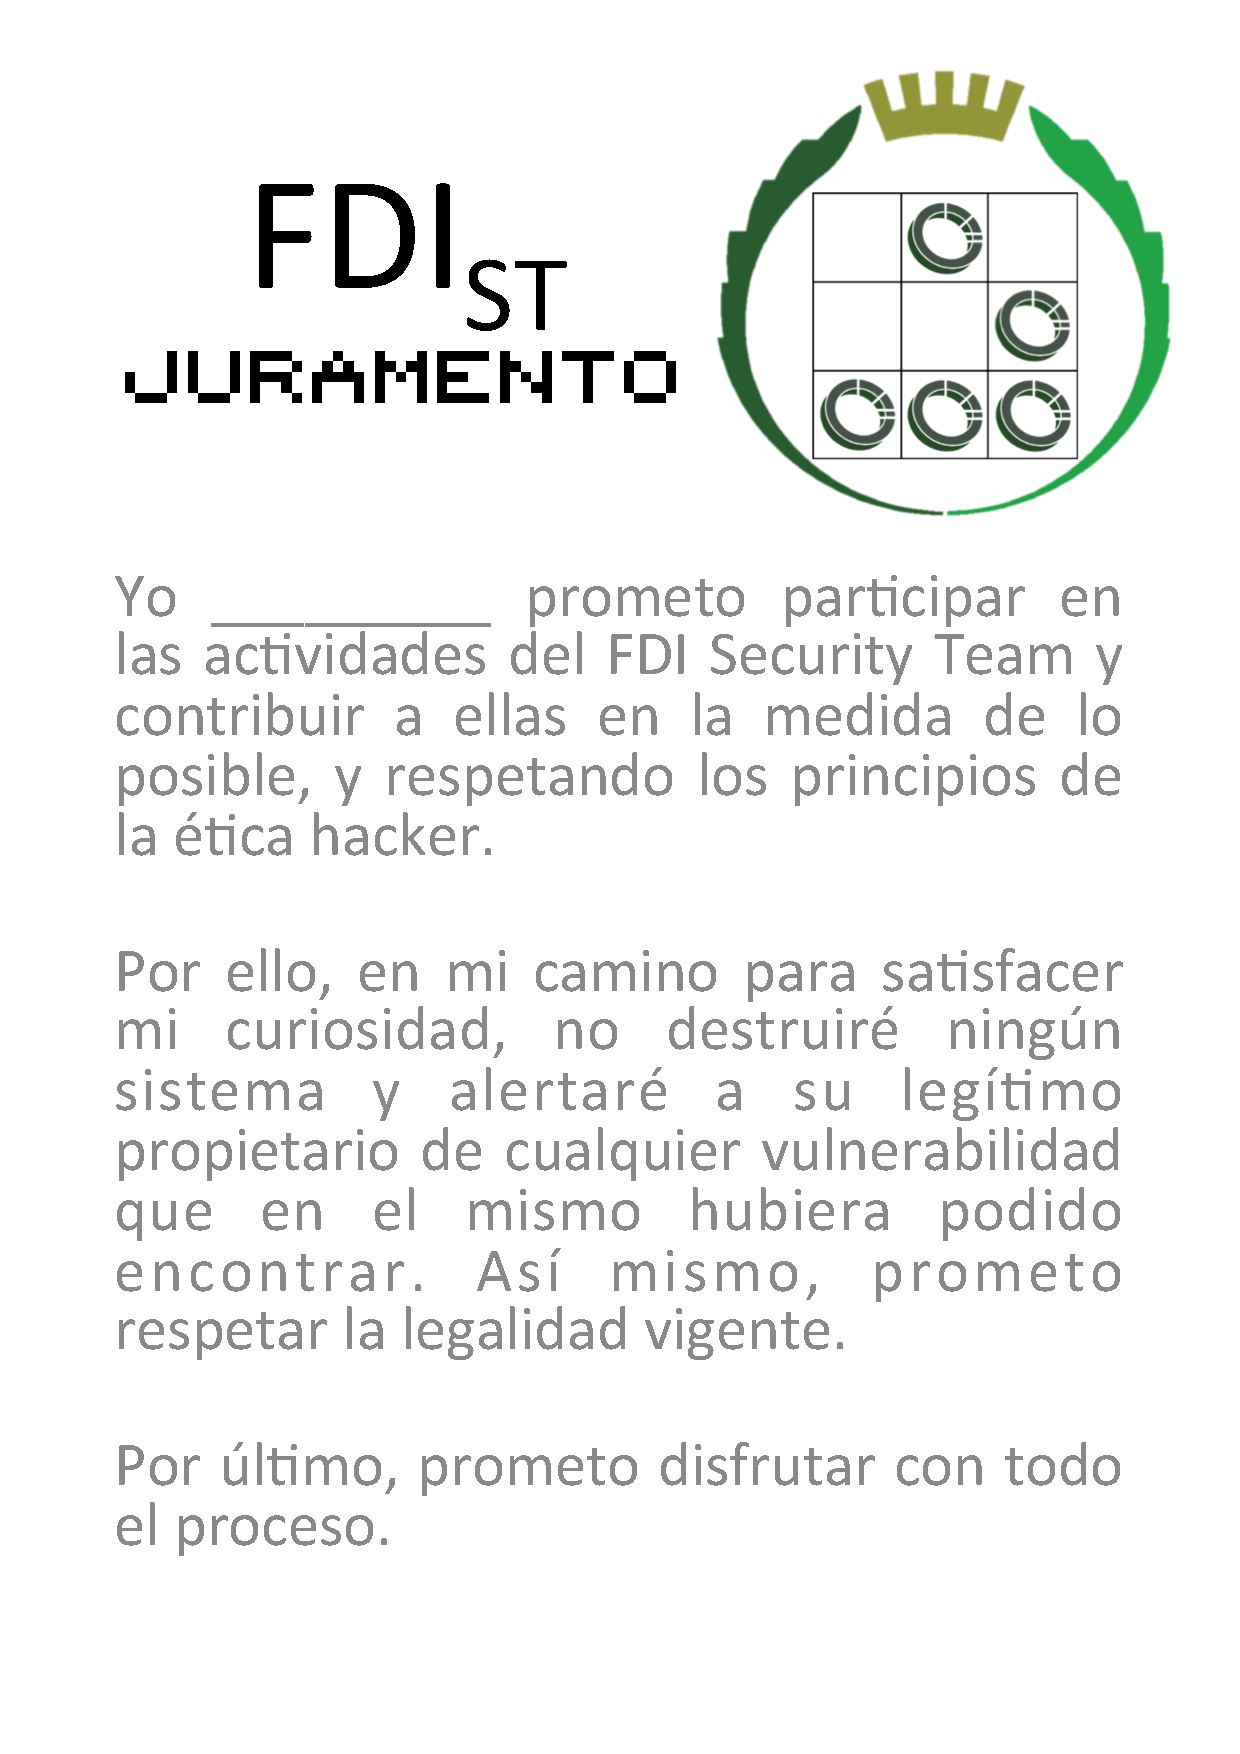
\includegraphics[width=0.93 \textwidth]{Media/Juramento.pdf}
\end{figure}
%\input{Capitulos/8.El_manifiesto_Hacker.tex}
\newpage
\vspace*{\fill} % Para que lo escriba al final de la página
\doclicenseThis %done

\end{document}